
\section{Case Study}
As we mentioned in the \S4, despite the improvement of memory structure, the performance of experiments on simulated dialogues has a decrease compared with original dialogues, possibly due to the limited role-play capability of LLMs. We will present some cases to illustrate these limitations. 

\subsection{Hallucination}
In the simulated dialogue experiments, we found that when engaging in role-playing, LLMs tend to make unfounded elaborations based on previously mentioned symptoms or events. In the example presented in Table~\ref{tab:hallucination}, the patient only mentioned a past tendency toward self-harm in the original dialogue in D$^4$, which was promptly stopped by friends. However, in the simulated dialogue, the patient agent exaggerated the description on this by stating "It doesn't happen very often, about once a month or so".

\begin{table}[!h]
    \centering
    \begin{tabular}{m{0.3\linewidth}m{0.6\linewidth}}
    \toprule
         Original Dialogue & I occasionally \textcolor{orange}{have urges to self-harm}, but my friends \textcolor{orange}{have stopped me in time}. \\ 
    \midrule
    \midrule
         Simulated Question & Could you tell me more about how often and in what ways you self-harm? \\
    \midrule
         Simulated Response & It doesn't happen very often, about \textcolor{orange}{once a month or so}. \\
    \bottomrule
    \end{tabular}
    \caption{\textbf{Example of Hallucination}. The content is translated from Chinese utterances.}
    \label{tab:hallucination}
\end{table}


\subsection{Repetition}
We also observed that when generating dialogues, large models tend to replicate the format and content of previous exchanges, leading to repetitive phrasing or responses. This causes the current phase of the conversation to mirror earlier ones, and subsequent dialogues to mirror the current phase, resulting in the entire conversation using similar structures and getting stuck on certain topics. The example is represented in Table~\ref{tab:repetition}.

\begin{table}[!h]
    \centering
    \begin{tabular}{m{2cm}m{6cm}}
    \toprule
         Psychiatrist Agent & Mr. Lin, \textcolor{blue}{thank you for sharing} about the decrease in your social activities. Besides that, \textcolor{blue}{have you noticed} any mood swings or feelings of depression recently? Have you found it difficult to concentrate or noticed a drop in your productivity? \textcolor{blue}{These changes are important for me to better understand and assess your mental state}. \\
    \midrule
         Patient Agent & \textcolor{orange}{Recently}, I've noticed that I'm not as socially active as I used to be. I'm no longer as enthusiastic about going out or meeting up with friends. This change has been tough for me, and I do feel a bit lonely because of it. \\
    \midrule
         Psychiatrist Agent & Mr. Lin, \textcolor{blue}{thank you for sharing}. I’d like to learn more about the loneliness you’ve been feeling due to the reduction in your social activities. \textcolor{blue}{Have you noticed} a lack of opportunities to connect with friends, or do you feel that this decrease has added extra stress and a sense of isolation? \textcolor{blue}{These details are important for us to better understand your emotional well-being}. \\
    \midrule
         Patient Agent& \textcolor{orange}{Recently}, I've been feeling lonely and stressed. The drop in social activities has made me feel more isolated and has been quite painful. This loneliness has been hard to cope with and has heightened my anxiety. \\
    \bottomrule
    \end{tabular}
    \caption{\textbf{Example of Repetition}. The content is translated from Chinese utterances.}
    \label{tab:repetition}
\end{table}



\subsection{Language Style}
Owing to the lack of original dialogue for a single patient, the data available for LLMs to learn from is also constrained. Consequently, in simulated dialogues, the models often fail to accurately capture the patient's language style and may even use professional medical terminology in their first session, which doesn't align with the patient's identity when describing symptoms, as Table~\ref{tab:language style} represents. This could lead to potential diagnostic inaccuracies.

\begin{table}[!h]
    \centering
    \begin{tabular}{m{2cm}m{6cm}}
    \toprule
         Patient Agent & Hello, Dr. Bernard. My name is Xiaohong, and I’m \textcolor{orange}{11 years old}, currently a primary school student. Lately, I've noticed a decline in my memory, and I've been experiencing some \textcolor{orange}{psychomotor agitation} and \textcolor{orange}{retardation}. I’m reaching out for help. \\
    \midrule
         Psychiatrist Agent & Hello, Xiaohong. Thank you for sharing this information with me. \\
    \bottomrule
    \end{tabular}
    \caption{\textbf{Example of Language Style}. The content is translated from Chinese utterances.}
    \label{tab:language style}
\end{table}


\section{Data Characteristics of D$^4$}
D$^4$ is a Chinese depression diagnosis dataset, the overall statistics can be shown as Table~\ref{tab:data characteristic}. The distribution of the User Portrait is presented in Figure~\ref{fig:portrait distribution train} and Figure~\ref{fig:portrait distribution test}.

\begin{table}[htbp]
    \centering
    \small
    \begin{tabular}{cccc}
    \toprule
    \textbf{Category}&\textbf{Total}&\textbf{Patient}&\textbf{Doctor} \\
    \midrule
        Dialogues & 1339 & - & - \\
    \midrule
        Avg. turns & 21.6 & - & - \\
    \midrule
        Workers & 201 & 127 & 74 \\
    \midrule
        Avg. utterances per dialogue & 60.9 & 30.9 & 29.9 \\
    \midrule
        Avg. tokens per dialogue & 877.6 & 381.8 & 495.8 \\
    \midrule
        Avg. tokens per utterance & 14.4 & 12.3 & 16.6 \\
    \bottomrule
    \end{tabular}
    \caption{\textbf{Overall Statistics of D$^4$.}}
    \label{tab:data characteristic}
\end{table}

\begin{figure}[!t]
    \centering
    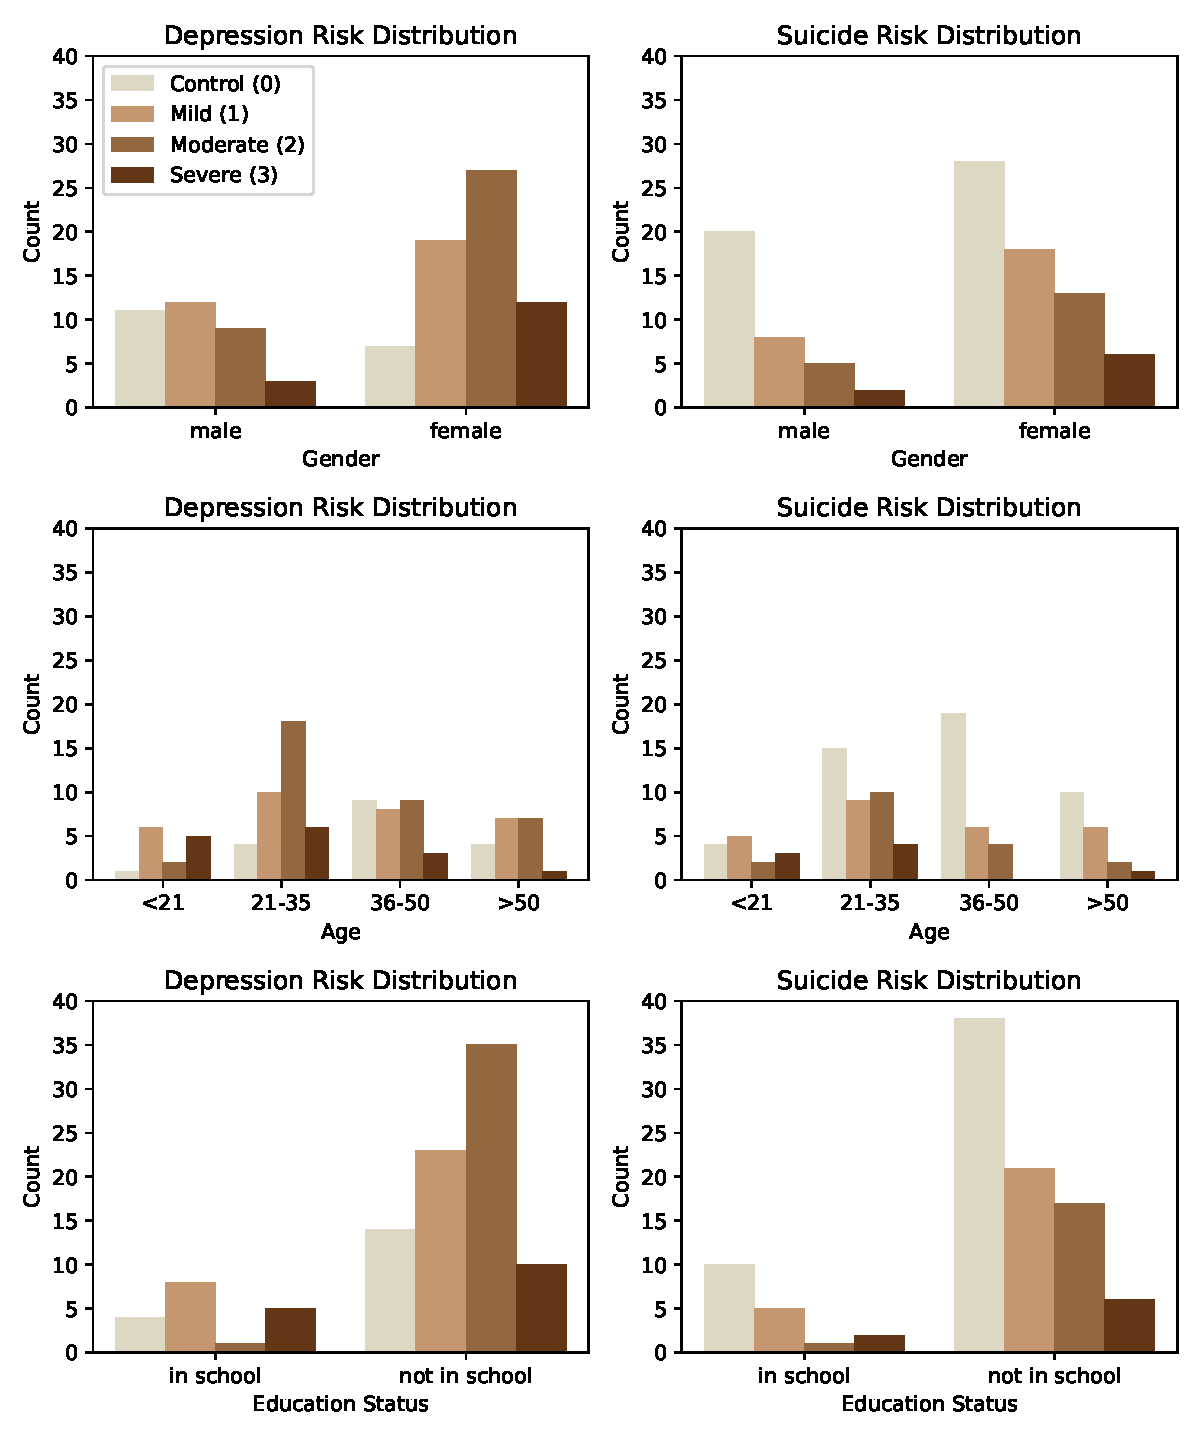
\includegraphics[width=\linewidth]{fig/distribution_train.pdf}
    \caption{\textbf{The Distribution of Portrait on Train Set.}}
    \label{fig:portrait distribution train}
\end{figure}


\begin{figure}[!t]
    \centering
    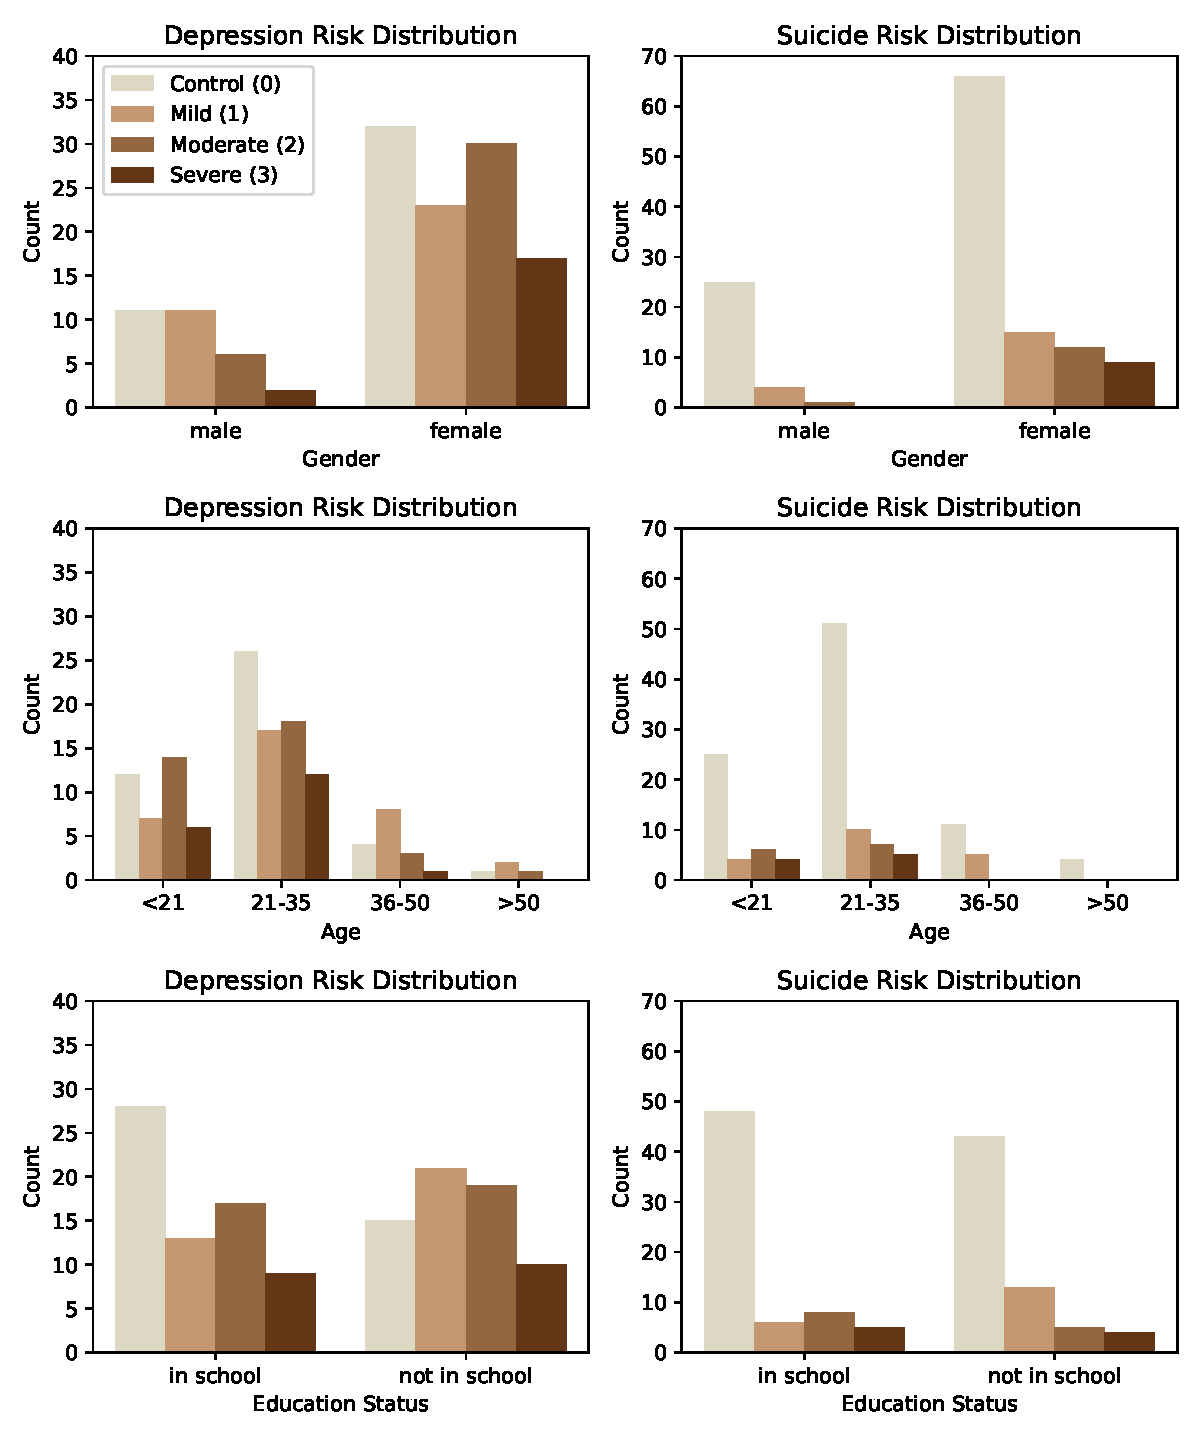
\includegraphics[width=\linewidth]{fig/distribution_test.pdf}
    \caption{\textbf{The Distribution of Portrait on Test Set.}}
    \label{fig:portrait distribution test}
\end{figure}


% \section{Ethical Considerations}

\section{Ethics and Broader Impact Statement}

    \paragraph{Data Privacy}
    The data used in this paper comes from a previously published dataset, and all evaluation metrics are based on objective computations. Although experts' evaluations could be included in future work, this study currently raises little ethical concerns. Any content related to user privacy has been appropriately processed for disclosure in the paper and supplementary files.

    \paragraph{Intended Use}
    \system~system is designed to conduct simulated depression diagnosis dialogues and assess both the depression risk and suicide risk of potential patients. The system can be subsequently be deployed as interactive system for intern psychiatrist training and preliminary screening for potential patients.

    \paragraph{Potential Misuse}
    Since the \system~system is designed to conduct the preliminary screening, the psychiatrist agent is equipped with diagnosis knowledge collected from ICD-11. Therefore, the psychiatrist agent is not appropriate to provide medical suggestions, which might lead to misinterpretation or misuse of the information provided. Instead, the psychiatrist agent is intended to offer general guidance and support during the initial stages of assessment, while encouraging users to seek professional medical advice from a qualified healthcare provider for any specific concerns or diagnoses. This approach ensures that the system serves as a complementary tool, rather than a substitute for professional medical consultation.

    \paragraph{Environmental Impact}
    Our \system~can be utilized for potential patient who are suffering from depressive mood. Currently, mental health issues, especially depressive disorder, are prevalent, yet a significant number of individuals fail to recognize their own mental health problems promptly or seek timely treatment. The \system~system, constructed as a future platform accessible across three interfaces, aspires to serve as an efficient tool for enhancing psychiatrists' professional expertise, offering the public convenient and highly confidential diagnostic assessments, and improving diagnostic accuracy across the mental health field. Through these contributions, we hope to contribute to the improvement of global mental health.

\section{Limitation and Future Work}
Our research has limitations that can be further improved in future work.

While the Agent Mental Clinic (AMC) system has shown promising potential in enhancing depression diagnosis through simulated dialogues, there are areas that warrant further development. The system’s effectiveness is currently shaped by its reliance on the D4 dataset, which may limit its applicability in diverse cultural and linguistic contexts. Additionally, the accuracy of role-playing within the system reflects the inherent challenges of current large language models (LLMs) in fully capturing the details of depressive symptoms, which can sometimes result in less precise simulations. Although the memory retrieval module has seen improvements, it still encounters difficulties in fully encompassing the complexities of mental health diagnoses. Moreover, the absence of real-time expert feedback may affect the system's ability to adapt to particularly complex cases.

Looking ahead, future efforts would focus on broadening the AMC system's adaptability to various cultural settings, further refining the role-playing capabilities of LLMs, and advancing the sophistication of memory retrieval methods. Integrating real-time expert feedback and extending the system's application to additional mental health conditions could enhance its accuracy, cultural sensitivity, and overall comprehensiveness in diagnostic processes.


% the insufficiency of diagnosis accuracy on simulated dialogues ; high cost (? ; limited dataset quality due to constrained resources ; inadequate evaluation of dialogue generation quality (and diagnosis accuracy)

% implement multi-port access for real users ; incorporate a feature for diagnosing specific symptoms ; enhance the system's ability to simulate and implement different language styles, providing a better experience for users ; consider more efficient memory storage formats to reduce costs






\section{Reproducibility Checklist}
This paper:
\begin{itemize}
    \item Includes a conceptual outline and/or pseudocode description of AI methods introduced: \textbf{yes}
    \item Clearly delineates statements that are opinions, hypothesis, and speculation from objective facts and results: \textbf{yes}
    \item Provides well marked pedagogical references for less-familiare readers to gain background necessary to replicate the paper: \textbf{yes}
\end{itemize}

Does this paper make theoretical contributions? \textbf{no}

Does this paper rely on one or more datasets? \textbf{yes}

If yes, please complete the list below.
\begin{itemize}
    \item A motivation is given for why the experiments are conducted on the selected datasets \textbf{yes}
    \item All novel datasets introduced in this paper are included in a data appendix. \textbf{NA}
    \item All novel datasets introduced in this paper will be made publicly available upon publication of the paper with a license that allows free usage for research purposes. \textbf{NA}
    \item All datasets drawn from the existing literature (potentially including authors’ own previously published work) are accompanied by appropriate citations. \textbf{yes}
    \item All datasets drawn from the existing literature (potentially including authors’ own previously published work) are publicly available. \textbf{yes}
    \item All datasets that are not publicly available are described in detail, with explanation why publicly available alternatives are not scientifically satisficing. \textbf{yes}
\end{itemize}

Does this paper include computational experiments? yes
If yes, please complete the list below.
\begin{itemize}
    \item Any code required for pre-processing data is included in the appendix. \textbf{yes}
    \item All source code required for conducting and analyzing the experiments is included in a code appendix. \textbf{yes}
    \item All source code required for conducting and analyzing the experiments will be made publicly available upon publication of the paper with a license that allows free usage for research purposes. \textbf{yes}
    \item All source code implementing new methods have comments detailing the implementation, with references to the paper where each step comes from. \textbf{yes}
    \item If an algorithm depends on randomness, then the method used for setting seeds is described in a way sufficient to allow replication of results. \textbf{yes}
    \item This paper specifies the computing infrastructure used for running experiments (hardware and software), including GPU/CPU models; amount of memory; operating system; names and versions of relevant software libraries and frameworks. \textbf{yes}
    \item This paper formally describes evaluation metrics used and explains the motivation for choosing these metrics. \textbf{yes}
    \item This paper states the number of algorithm runs used to compute each reported result. \textbf{yes}
    \item Analysis of experiments goes beyond single-dimensional summaries of performance (e.g., average; median) to include measures of variation, confidence, or other distributional information. \textbf{yes}
    \item The significance of any improvement or decrease in performance is judged using appropriate statistical tests (e.g., Wilcoxon signed-rank). \textbf{yes}
    \item This paper lists all final (hyper-)parameters used for each model/algorithm in the paper’s experiments. \textbf{yes}
    \item This paper states the number and range of values tried per (hyper-) parameter during development of the paper, along with the criterion used for selecting the final parameter setting. \textbf{yes}
\end{itemize}
